% Options for packages loaded elsewhere
\PassOptionsToPackage{unicode}{hyperref}
\PassOptionsToPackage{hyphens}{url}
\PassOptionsToPackage{dvipsnames,svgnames,x11names}{xcolor}
%
\documentclass[11pt]{article}
\usepackage{amsmath,amssymb}
\usepackage{lmodern}
\usepackage{iftex}
\ifPDFTeX
  \usepackage[T1]{fontenc}
  \usepackage[utf8]{inputenc}
  \usepackage{textcomp}
\fi
\IfFileExists{microtype.sty}{\usepackage[]{microtype}\UseMicrotypeSet[protrusion]{basicmath}}{}
\makeatletter
\@ifundefined{KOMAClassName}{%
  \IfFileExists{parskip.sty}{\usepackage{parskip}}{%
    \setlength{\parindent}{0pt}\setlength{\parskip}{6pt plus 2pt minus 1pt}}
}{\KOMAoptions{parskip=half}}
\makeatother
\usepackage{xcolor}
\IfFileExists{xurl.sty}{\usepackage{xurl}}{}
\IfFileExists{bookmark.sty}{\usepackage{bookmark}}{\usepackage{hyperref}}
\hypersetup{
  pdftitle={Final Report Template, Architecture Document},
  pdfauthor={Team name},
  colorlinks=true,
  linkcolor={RoyalBlue},
  filecolor={Maroon},
  citecolor={Blue},
  urlcolor={Blue}}
\urlstyle{same}
\usepackage[a4paper,margin=2.4cm]{geometry}
\usepackage{longtable,booktabs,array}
\usepackage{calc}
\usepackage{graphicx}
\makeatletter
\def\maxwidth{\ifdim\Gin@nat@width>\linewidth\linewidth\else\Gin@nat@width\fi}
\def\maxheight{\ifdim\Gin@nat@height>\textheight\textheight\else\Gin@nat@height\fi}
\makeatother
\setkeys{Gin}{width=\maxwidth,height=\maxheight,keepaspectratio}
\setlength{\emergencystretch}{3em}
\providecommand{\tightlist}{\setlength{\itemsep}{0pt}\setlength{\parskip}{0pt}}
\setcounter{secnumdepth}{-\maxdimen}
\usepackage{newunicodechar}
\usepackage{textcomp}
\usepackage{amssymb}
\newunicodechar{°}{\textdegree}
\newunicodechar{₂}{\textsubscript{2}}
\newunicodechar{→}{\ensuremath{\rightarrow}}
\newunicodechar{≤}{\ensuremath{\leq}}
\newunicodechar{≥}{\ensuremath{\geq}}
\newunicodechar{≈}{\ensuremath{\approx}}
\newunicodechar{✓}{\ensuremath{\checkmark}}
\newunicodechar{–}{--}
\newunicodechar{—}{---}
\usepackage{etoolbox}
\AtBeginEnvironment{longtable}{\footnotesize}
\AtBeginEnvironment{tabular}{\footnotesize}
\usepackage{fancyhdr}
\pagestyle{fancy}\fancyhf{}
\rhead{\small D7065E\,--\,Architecture Document}
\lhead{\small Final Report (template)}
\cfoot{\thepage}
\renewcommand{\headrulewidth}{0.4pt}
\usepackage{titlesec}
\titleformat{\section}{\Large\bfseries}{\thesection}{0.6em}{}
\titleformat{\subsection}{\large\bfseries}{\thesubsection}{0.5em}{}
\usepackage{microtype}
\usepackage{pgfplots}
\pgfplotsset{compat=1.16}
\setlength{\emergencystretch}{2em}

% --- template helpers -------------------------------------------------------
\definecolor{guidegray}{gray}{0.42}
% Grey guidance note: what this section must contain. Delete before submission.
\newcommand{\guidance}[1]{{\color{guidegray}\small\textit{#1}}\par\vspace{0.3em}}
% A slot to be replaced with the team's own prose.
\newcommand{\fillin}[1]{\par\noindent\fbox{\parbox{\dimexpr\linewidth-2\fboxsep-2\fboxrule}{\color{guidegray}\textit{[#1]}}}\par\vspace{0.4em}}
% A placeholder where a rendered diagram should be inserted.
\newcommand{\diagramslot}[1]{\par\begin{center}\fbox{\parbox[c][2.6cm][c]{0.82\linewidth}{\centering\color{guidegray}\textit{[Insert: #1]}}}\end{center}\par}
% ---------------------------------------------------------------------------

\title{Final Report, Architecture Document}
\usepackage{etoolbox}
\makeatletter
\providecommand{\subtitle}[1]{\apptocmd{\@title}{\par {\large #1 \par}}{}{}}
\makeatother
\subtitle{D7065E, fill-in template}
\author{Team name: First member \& Second member}
\date{}

\begin{document}

{\setlength{\fboxsep}{7pt}\setlength{\fboxrule}{0.6pt}%
\begin{center}
\fbox{\fbox{\parbox{0.88\linewidth}{%
\textbf{How to use this template.} This is the \textbf{skeleton} of the final
architecture document. Each section carries a short \textcolor{guidegray}{\textit{grey
guidance note}} describing what it must contain, and \textcolor{guidegray}{\textit{[bracketed
slots]}} to replace with the project's own content. Replace every slot, insert the
diagrams where marked, and \textbf{delete the guidance notes} before submission.
The companion \emph{guide} explains the reasoning behind each section; the worked
\emph{example} shows a complete version at the grade-5 standard. Quality of reasoning
matters more than length: a small, well-justified, well-evaluated system scores higher
than a large one that cannot be explained.%
}}}
\end{center}}

\vspace{1.2em}

\begin{center}
{\LARGE Project Title\par}
\vspace{0.5em}
{\large D7065E, Architecture Document\par}
\vspace{1em}
{Team name: First member \& Second member\par}
\end{center}

\vspace{1.2em}

{
\hypersetup{linkcolor=black}
\setcounter{tocdepth}{3}
\tableofcontents
}

\section{1. Summary}

\guidance{One short paragraph: what the system does and the single guiding
principle that threads through the design. Then the summary table, and a brief note
of what changed since the Week 2 proposal and why.}

\fillin{Write the one-paragraph summary here.}

\begin{longtable}[]{@{}
  >{\raggedright\arraybackslash}p{(\columnwidth - 2\tabcolsep) * \real{0.35}}
  >{\raggedright\arraybackslash}p{(\columnwidth - 2\tabcolsep) * \real{0.65}}@{}}
\toprule
\textbf{Field} & \textbf{Value} \\
\midrule
\endhead
\textbf{Project title} & \\
\textbf{Team members} & \\
\textbf{Use case} & \\
\textbf{Repository} & \\
\textbf{Version / date} & \\
\bottomrule
\end{longtable}

\textbf{Changes since the proposal.}
\fillin{List the design changes made since the proposal, and the evidence that
forced each one. If nothing changed, state that and say why.}

\section{2. Use case and building context}

\guidance{Describe the building and what BuildSim provides (rooms, sensors,
actuators, 3D view). State the use case and the tension or objective that makes the
autonomous decision non-trivial. BuildSim holds the shared building state; this
project provides the physics, the intelligence, and the control around it.}

\fillin{Describe the use case and the building context here.}

\section{3. Requirements}

\guidance{List functional and non-functional requirements with stable IDs, so each
can be traced to a test in the test plan and to results in the evaluation. Keep them
verifiable (avoid ``fast'' or ``reliable'' without a number).}

\begin{longtable}[]{@{}
  >{\raggedright\arraybackslash}p{(\columnwidth - 4\tabcolsep) * \real{0.12}}
  >{\raggedright\arraybackslash}p{(\columnwidth - 4\tabcolsep) * \real{0.58}}
  >{\raggedright\arraybackslash}p{(\columnwidth - 4\tabcolsep) * \real{0.30}}@{}}
\toprule
\textbf{ID} & \textbf{Requirement} & \textbf{How it is verified} \\
\midrule
\endhead
FR-1 & & \\
FR-2 & & \\
NFR-1 & & \\
NFR-2 & & \\
\bottomrule
\end{longtable}

\section{4. Architecture}

\subsection{4.1 Context diagram (C4 Level 1)}

\guidance{The system as a single box, with the people and external systems it
interacts with (including BuildSim). One paragraph of narrative explaining the
boundaries and the main interactions.}

\diagramslot{Context diagram (C4 Level 1)}

\fillin{Narrative for the context diagram.}

\subsection{4.2 Container diagram (C4 Level 2)}

\guidance{Open the system into its separately-running parts (sensor services,
autonomous service, actuators, storage, dashboard) and how they communicate. Explain
why the system is split this way.}

\diagramslot{Container diagram (C4 Level 2)}

\fillin{Narrative for the container diagram.}

\subsection{4.3 Component diagram (C4 Level 3)}

\guidance{Zoom into one container that is worth explaining (often the autonomous
service) and show its internal components and their responsibilities.}

\diagramslot{Component diagram (C4 Level 3)}

\fillin{Narrative for the component diagram.}

\subsection{4.4 Design decisions and alternatives}

\guidance{The core of the architecture grade. For each significant decision, state
the choice, the alternatives considered, and the evidence or reasoning for choosing
it over them. A decision with no rejected alternative is not yet justified.}

\begin{longtable}[]{@{}
  >{\raggedright\arraybackslash}p{(\columnwidth - 4\tabcolsep) * \real{0.25}}
  >{\raggedright\arraybackslash}p{(\columnwidth - 4\tabcolsep) * \real{0.35}}
  >{\raggedright\arraybackslash}p{(\columnwidth - 4\tabcolsep) * \real{0.40}}@{}}
\toprule
\textbf{Decision} & \textbf{Alternatives considered} & \textbf{Why this one} \\
\midrule
\endhead
 & & \\
 & & \\
 & & \\
\bottomrule
\end{longtable}

\section{5. Interfaces and data contracts}

\guidance{The contracts between components: API endpoints and/or message topics,
with payload schemas and an example message. Precise enough that a component could be
re-implemented from this section alone.}

\fillin{Define the interfaces and data contracts here (endpoints/topics, schemas,
example payloads).}

\section{6. Simulating the sensor values (the physical model)}

\guidance{How sensor values are produced. State the per-room physical model
(temperature heat balance, CO₂ from occupancy and ventilation) and, critically, how
actuator commands feed back so the control loop closes. Include the occupancy model
(for example, a head-count per room sampled conditional on room type and time of day).
Give the governing equations.}

\fillin{Describe the physical and occupancy models, with equations, here.}

\section{7. Autonomous services and data pipeline}

\subsection{7.1 The autonomous service}

\guidance{The decision logic: inputs, the algorithm or rules, and outputs. Rule-based
control is fully acceptable if justified; if a learned model is used, explain training,
data, and the fallback when data is thin.}

\fillin{Describe the autonomous service here.}

\subsection{7.2 The data pipeline}

\guidance{How readings are collected, stored, and served to the autonomous service
and the dashboard. State what is retained and for how long.}

\fillin{Describe the data pipeline here.}

\section{8. Behaviour}

\subsection{8.1 Key scenario (dynamic diagram)}

\guidance{Walk one important scenario end-to-end (for example, a room filling up) as
a C4 dynamic / sequence diagram, with a short narrative of the message order.}

\diagramslot{Dynamic / sequence diagram for the key scenario}

\fillin{Narrative for the key scenario.}

\subsection{8.2 Process lifecycle (state diagram)}

\guidance{The lifecycle of a key process or zone (for example, setback $\rightarrow$
active $\rightarrow$ fault), as a state diagram with the transitions.}

\diagramslot{State diagram for the process lifecycle}

\fillin{Narrative for the state diagram.}

\section{9. Deployment and component view}

\guidance{Where each process runs (edge nodes, a server, BuildSim) and how they are
connected. Note where computation belongs and why.}

\diagramslot{Deployment diagram}

\fillin{Narrative for the deployment view.}

\section{10. Test plan}

\guidance{The tests that verify the requirements, including stress and failure tests
(a sensor that lies, a process that dies, a flood of readings). Each row should trace
back to a requirement ID from Section 3.}

\begin{longtable}[]{@{}
  >{\raggedright\arraybackslash}p{(\columnwidth - 6\tabcolsep) * \real{0.16}}
  >{\raggedright\arraybackslash}p{(\columnwidth - 6\tabcolsep) * \real{0.40}}
  >{\raggedright\arraybackslash}p{(\columnwidth - 6\tabcolsep) * \real{0.19}}
  >{\raggedright\arraybackslash}p{(\columnwidth - 6\tabcolsep) * \real{0.25}}@{}}
\toprule
\textbf{ID} & \textbf{Test} & \textbf{Requirement} & \textbf{Expected result} \\
\midrule
\endhead
T-1 & & & \\
T-2 & & & \\
T-3 (stress) & & & \\
\bottomrule
\end{longtable}

\section{11. Evaluation and results}

\guidance{The evidence that the system works, measured, not asserted. Charts and
tables of results, compared against the requirements. Include an honest reading of
where the numbers are weak. The plot below is a pgfplots placeholder, replace the
coordinates with real data.}

\begin{center}
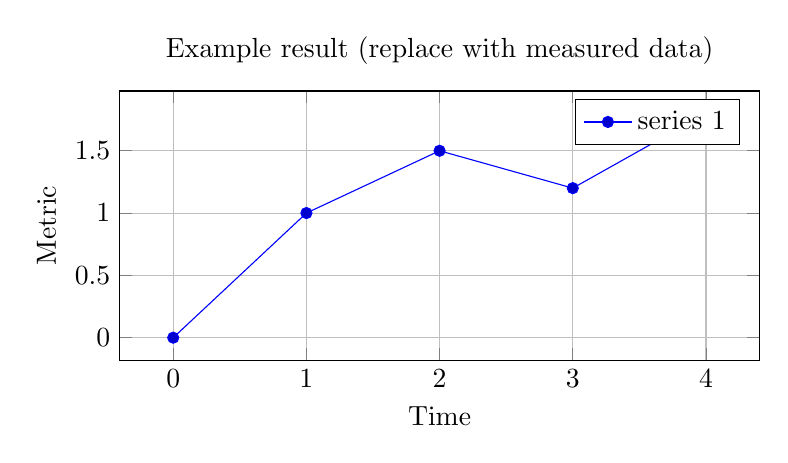
\begin{tikzpicture}
\begin{axis}[width=0.8\linewidth,height=5cm,xlabel={Time},ylabel={Metric},
  title={Example result (replace with measured data)},grid=both,
  legend pos=north east]
\addplot coordinates {(0,0) (1,1) (2,1.5) (3,1.2) (4,1.8)};
\legend{series 1}
\end{axis}
\end{tikzpicture}
\end{center}

\fillin{Present and interpret the results here.}

\section{12. Dashboard}

\guidance{What the dashboard shows and how it overlays state and decisions on the
BuildSim 3D view. Include a screenshot.}

\diagramslot{Dashboard screenshot}

\fillin{Describe the dashboard here.}

\section{13. Risks and critical reflection}

\guidance{An honest account of weaknesses, trade-offs, and what would be done with
more time. Critical thinking is graded here: naming a real limitation scores better
than claiming there are none.}

\fillin{Reflect critically on the design here: limitations, trade-offs, and next
steps.}

\section{Checklist before submission}

\begin{itemize}
\tightlist
\item All \textcolor{guidegray}{\textit{[bracketed slots]}} replaced with real content.
\item All grey guidance notes deleted.
\item All five diagrams inserted and referenced in the text (context, container, component, dynamic, deployment).
\item Every requirement in Section 3 traced to a test in Section 10.
\item Each design decision in Section 4.4 names a rejected alternative.
\item Evaluation backed by measured data, not assertions.
\item The document matches what was actually built.
\end{itemize}

\end{document}
